\chapter{异构数据并行计算}
\label{chap:heterogeneous-data-parallel-computing}

数据并行性是这样一种现象：要在数据集的不同部分上执行的计算彼此独立，因此
可以并行执行。许多应用都具有丰富的数据并行性，适合进行可扩展的并行执行；在
这种执行方式下，执行速度会随着系统中执行资源数量的增加而近似成比例地提高。
因此，并行程序员有必要熟悉数据并行性的概念，以及用于编写能够利用数据并行性的
代码的并行编程语言构造。本章将使用 CUDA C++ 语言构造开发一个简单的数据并行
程序。

\section{数据并行性}
\label{sec:data-parallelism}

现代软件应用运行缓慢时，问题通常来自数据——需要处理的数据太多。图像处理应用
会处理包含数百万乃至数万亿像素的图像或视频；科学应用会用数十亿个网格点模拟
流体动力学；分子动力学应用会模拟数千到数十亿个原子之间的相互作用；航空公司
排班则必须处理数千个航班、机组和机场登机口。通常，这些像素、粒子、网格点、
相互作用、航班等对象在很大程度上可以独立处理。

例如，在图像处理中，把彩色像素转换为灰度只需要该像素的数据；模糊图像时，把
每个像素的颜色与附近像素的颜色求平均，只需要一个很小的像素邻域。即使是看起来
需要全局信息的操作，例如求图像中所有像素的平均亮度，也可以拆分成许多能够独立
执行的较小计算。对不同数据片段进行这种相互独立的求值，就是数据并行性的基础。
编写数据并行代码，意味着围绕数据重新组织计算，使得到的独立计算能够并行执行，
从而更快——通常是快得多——地完成整体任务。

下面用一个彩色图像转灰度图像的例子说明数据并行性。图 \ref{fig:2-1} 中的左图
是由许多像素组成的彩色图像，每个像素包含红、绿、蓝三个分数值 $(r,g,b)$，取值
从 0（黑色）到 1（最大强度）。要把彩色图像转换为灰度图像，需要对每个像素
应用下面的加权和公式，计算亮度值 $L$：
\[
  L = r \times 0.299 + g \times 0.587 + b \times 0.114.
  \tag{2.1}
\]

\begin{figure}[htbp]
  \centering
  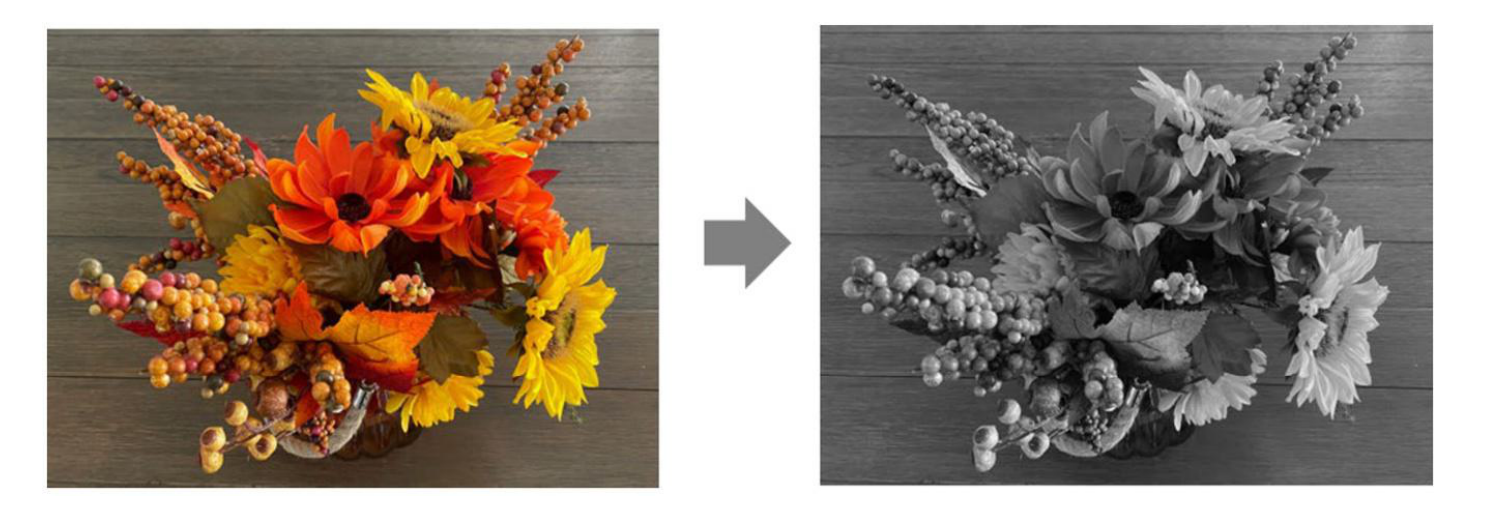
\includegraphics[width=\textwidth]{figs/ch2/2-1.png}
  \caption{彩色图像转换为灰度图像}
  \label{fig:2-1}
\end{figure}

\begin{quote}
\textbf{RGB 彩色图像表示}

在 RGB 表示中，图像的每个像素都表示为一个 $(r,g,b)$ 值元组。一行图像的格式
可以写成$(r\ g\ b)\ (r\ g\ b)\ \cdots\ (r\ g\ b)$.每个元组表示红光（R）、绿光（G）和蓝光（B）的混合。
也就是说，渲染像素时，每个像素的 $r$、$g$ 和 $b$ 值分别表示红、绿、蓝光源的强度，其中 0 表示暗，1 表示满强度。
\begin{center}
  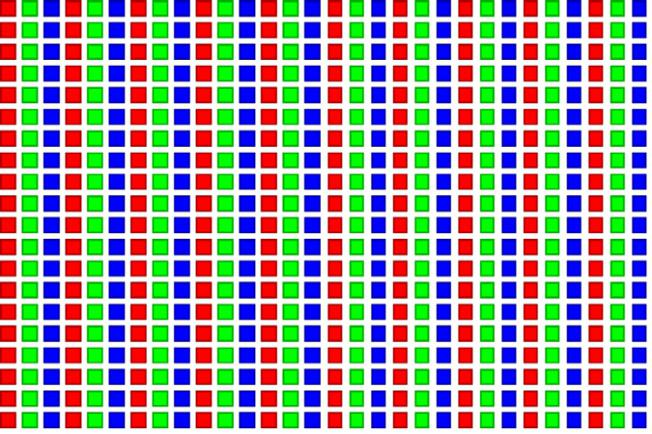
\includegraphics[width=0.5\textwidth]{figs/ch2/RGB.png}
\end{center}

\end{quote}

如果把输入看作由 RGB 值组成的数组 $I$，把输出看作对应的亮度值数组 $O$，就能
得到图 \ref{fig:2-2} 所示的简单计算结构。例如，$O[0]$ 是按照上面的公式对
$I[0]$ 中的 RGB 值求加权和得到的；$O[1]$ 由 $I[1]$ 中的 RGB 值得到；$O[2]$
由 $I[2]$ 中的 RGB 值得到，以此类推。这些逐像素计算彼此没有依赖，全部可以独立
执行。显然，彩色转灰度体现了丰富的数据并行性，因为现代图像通常包含数百万个
像素。当然，完整应用中的数据并行性可能更加复杂；本书很大一部分内容都致力于
教授发现并利用数据并行性所需的“并行思维”。

\begin{figure}[htbp]
  \centering
  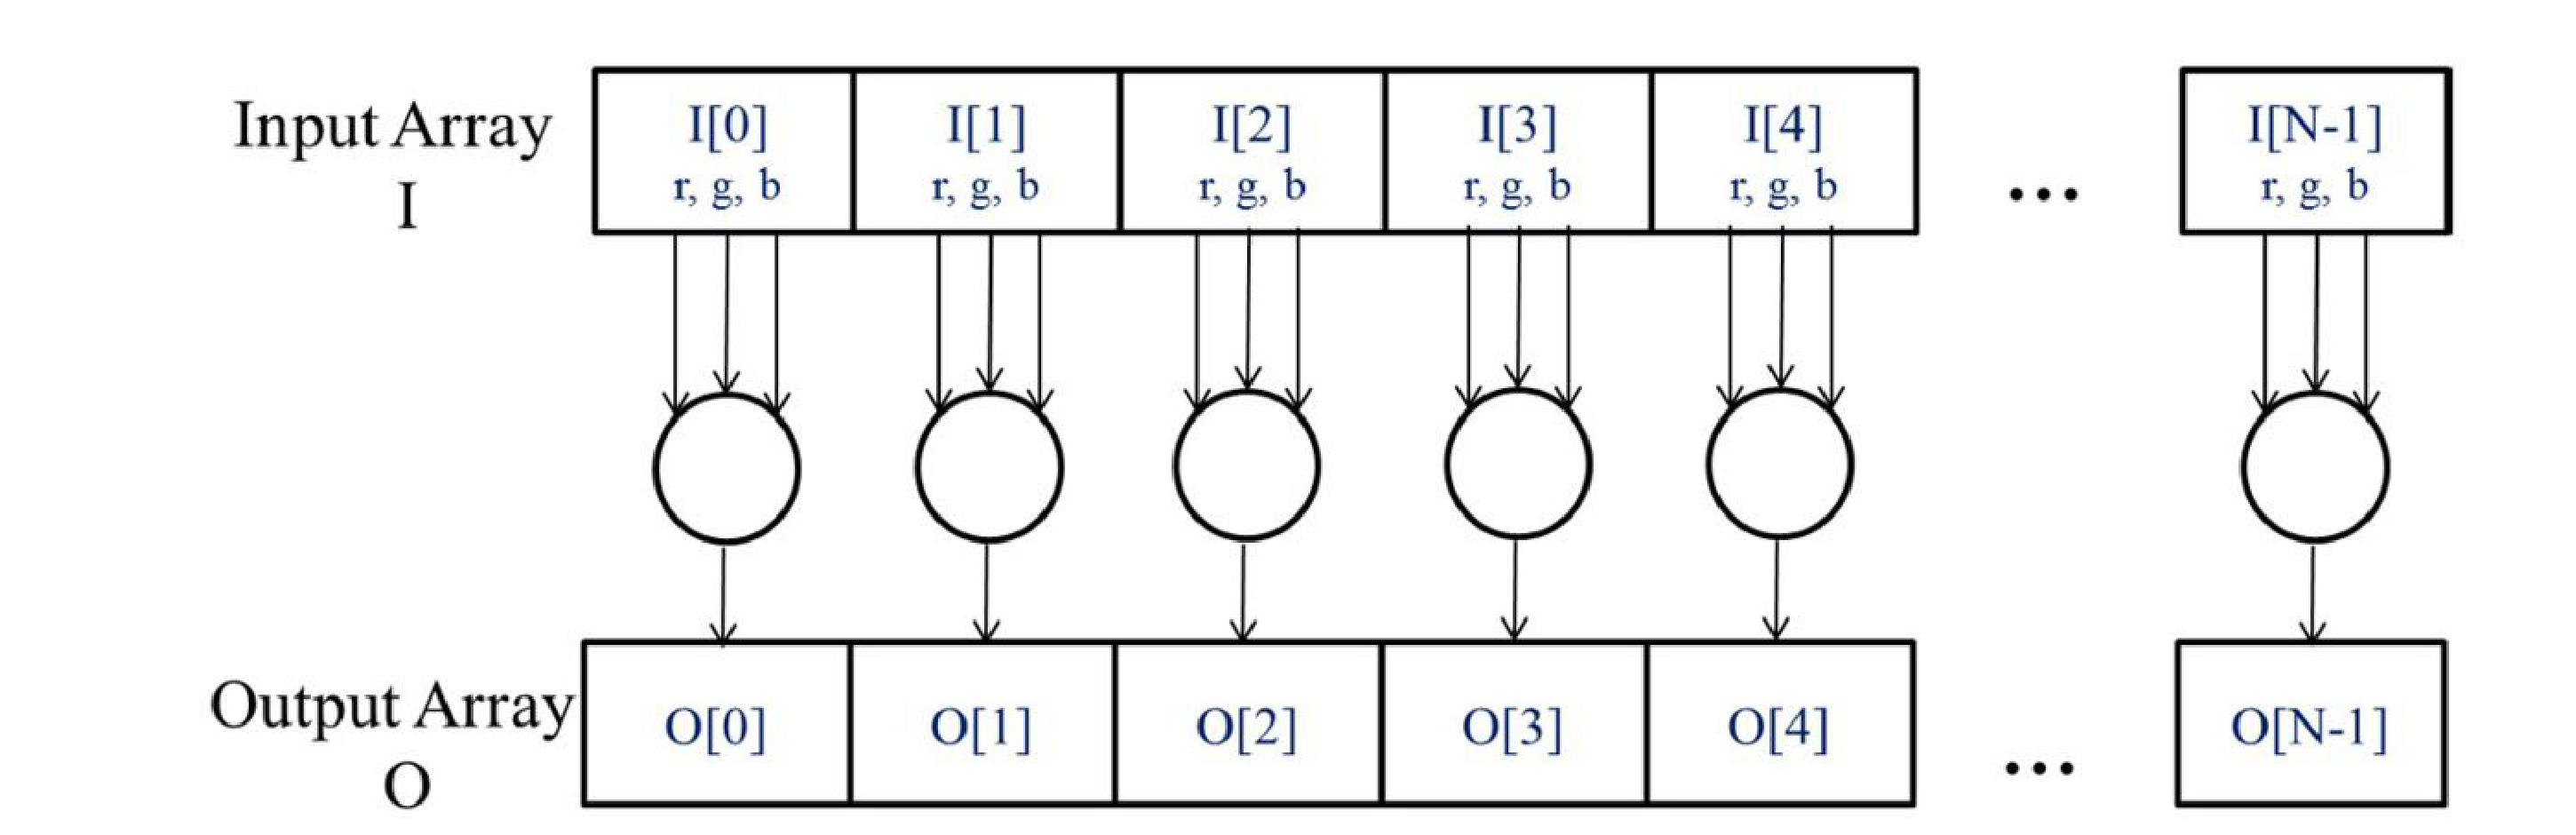
\includegraphics[width=\textwidth]{figs/ch2/2-2.png}
  \caption{彩色转灰度中的数据并行性：像素可以独立计算}
  \label{fig:2-2}
\end{figure}

\begin{quote}
\textbf{数据并行性与任务并行性}

数据并行性并不是并行编程中唯一使用的并行性类型。任务并行性也被广泛用于并行
编程。任务并行性通常通过对应用进行任务分解来暴露。例如，一个简单应用可能需要
执行向量加法和矩阵--向量乘法；这两项工作各自就是一个任务。如果两个任务可以
独立执行，就存在任务并行性。I/O 和数据传送也是常见的任务来源。

大型应用通常包含更多相互独立的任务，因此具有更多任务并行性。例如，在分子动力学
模拟器中，自然任务可能包括振动力计算、转动力计算、非键合力的邻居识别、非键合
力计算，以及速度和位置计算等。
\end{quote}

一般而言，数据并行性是并行程序获得性能提升的主要来源。面对大规模数据集，通常
可以找到充足的数据并行性，从而利用大规模并行处理器，并让应用性能随着每一代
拥有更多执行资源的硬件而提升；这种理想性质称为可扩展性（scalability）。不过，
任务并行性同样可能在实现性能目标时发挥重要作用。

\section{CUDA C++ 程序结构}
\label{sec:cuda-cpp-program-structure}

下一步是学习如何编写程序，在异构计算系统中利用数据并行性以获得更快的执行速度。
为了一般性地说明本书中的算法和技术，我们将使用 CUDA C++ 程序的代码示例。根据
我们的经验，基于 CUDA C++ 学到的概念很容易扩展到其他编程语言和平台。

CUDA C++\footnote{本书的代码示例为简洁起见使用 C 风格编程，并在需要时介绍 C++
特性。不过，读者应当注意，CUDA 编程已经逐渐转向 C++，以支持现代泛型编程和其他
面向对象的编程实践。} 在流行的 C++ 编程语言基础上，以少量新语法和库函数扩展
出面向异构计算系统的能力，使程序员能够针对同时包含 CPU 和 GPU 的系统编程。
顾名思义，CUDA C++ 建立在 NVIDIA 的 CUDA 平台之上。CUDA 目前是大规模并行
计算中最成熟的框架，已广泛用于高性能计算产业；在最常见的操作系统上，都能找到
编译器、调试器和性能分析器等重要工具。

CUDA C++ 程序的结构反映了计算机中主机（host，即 CPU）与一个或多个设备（device，
即 GPU）共存的情况。每个 CUDA C++ 源文件都可以混合包含主机代码和设备代码。
默认情况下，任何只包含主机代码的传统 C++ 程序也是一个 CUDA C++ 程序；可以在
任意源文件中加入设备代码。设备代码由特殊的 CUDA C++ 关键字明确标记，其中包括
函数（或称内核，kernel），其代码以数据并行方式执行。

图 \ref{fig:2-3} 展示了 CUDA C++ 程序的执行过程。执行从主机代码（CPU 串行代码）
开始，图中用一条代表线程的弯曲箭头表示。当调用内核——也就是设备代码的一部分
（图中的设备并行内核）——时，设备上会启动大量线程执行该内核。一次内核调用
所启动的全部线程统称为一个网格（grid）。这些线程是 CUDA 平台中并行执行的主要
载体。图 \ref{fig:2-3} 展示了两个线程网格的执行，每个网格又由多个线程块组成；
稍后会讨论网格和线程块的组织方式。当网格中的所有线程执行完毕后，网格终止，
执行回到主机，直到再次启动另一个网格。正如图中所暗示的，异构计算应用可以管理
CPU 和 GPU 的重叠执行，从而同时利用二者。

\begin{figure}[htbp]
  \centering
  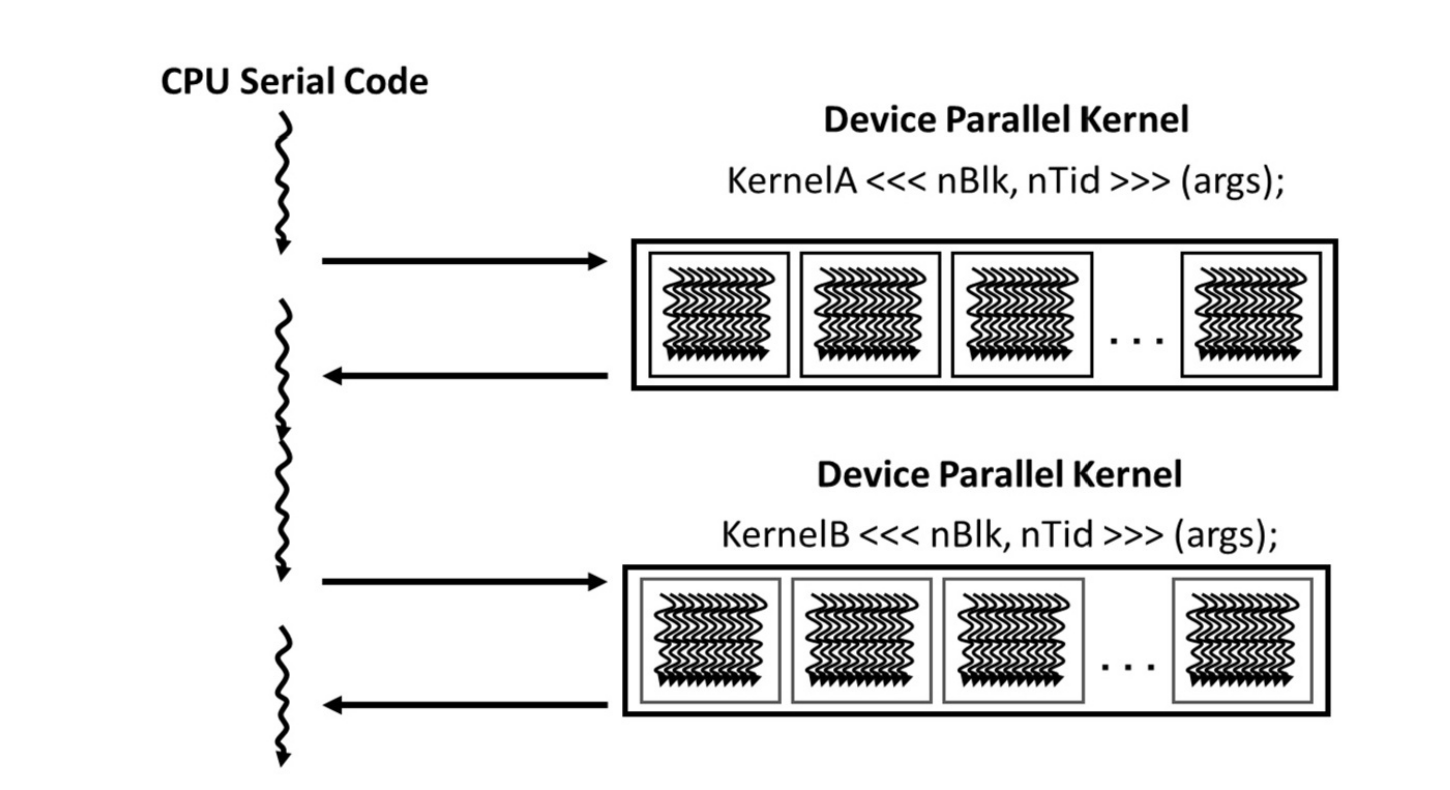
\includegraphics[width=\textwidth]{figs/ch2/2-3.png}
  \caption{CUDA 程序的执行过程}
  \label{fig:2-3}
\end{figure}

\begin{quote}
\textbf{线程}

线程是现代计算机中处理器执行顺序程序方式的一种简化视图。线程由程序代码、
当前正在执行的代码位置，以及变量和数据结构的值组成。从用户角度看，线程的执行
是顺序的。程序员可以使用源代码级调试器，逐条执行语句来监控线程进展，查看下一条
将要执行的语句，并在执行推进时检查变量和数据结构的值。

线程已经在编程中使用多年。如果程序员希望在应用中启动并行执行，就可以借助线程
库或专用语言创建并管理多个线程。在 CUDA 中，每个设备线程的执行同样是顺序的；
CUDA 程序通过调用内核函数启动并行执行，底层运行时机制则负责在设备上启动一个
线程网格，让线程并行处理数据。
\end{quote}

启动一个网格通常会生成大量线程，以利用数据并行性。在彩色转灰度的例子中，可以
让每个线程计算输出数组中的一个像素；此时，网格启动所生成的线程数应等于图像中
像素的数量。对于大图像，可能会生成数百万个线程。实践中，也可以让每个线程计算
多个输出像素，以提高执行和数据访问效率；本书后文会讨论这一点。由于硬件支持
高效的线程生成和调度，CUDA 程序员可以假设这些线程只需很少的时钟周期就能生成
和调度；传统 CPU 线程的生成和调度通常则需要数千个时钟周期。第 3 章将展示如何
实现彩色转灰度和图像模糊\textcolor{red}{内核}，本章为简洁起见使用向量加法作为贯穿示例。

\section{向量加法示例}
\label{sec:vector-addition-example}

向量加法可以说是最简单的数据并行计算，\textcolor{red}{是顺序编程中 ``Hello World'' 的并行
对应物}。在展示向量加法的内核代码之前，先回顾传统向量加法（主机代码）函数的
工作方式会很有帮助。图 \ref{fig:2-4} 展示了一个由 \code{main} 函数和向量加法
函数组成的简单 C++ 程序。

在本书的所有示例中，只要需要区分主机数据和设备数据，就会在主机使用的变量名
后加上 \code{_h}，在设备使用的变量名后加上 \code{_d}，以提醒自己这些变量的
预期用途。由于图 \ref{fig:2-4} 只有主机代码，因此其中只出现带 \code{_h} 后缀
的变量。

假设要相加的向量存放在数组 $A$ 和 $B$ 中，它们在 \code{main} 函数中分配并初始化；
输出向量存放在数组 $C$ 中，该数组也在 \code{main} 函数中分配。为简洁起见，图中
没有展示 \code{main} 函数如何分配和初始化 $A$、$B$、$C$ 的细节。这些数组的
指针，以及表示向量长度的变量 $N$，会传给 \code{vecAdd} 函数。注意，
\code{vecAdd} 的参数带有 \code{_h} 后缀，以强调它们由主机使用。

\begin{figure}[htbp]
  \centering
  \begin{lstlisting}[language=C++]
// Compute vector sum C_h = A_h + B_h
void vecAdd(float* A_h, float* B_h, float* C_h, int n) {
    for (int i = 0; i < n; ++i) {
        C_h[i] = A_h[i] + B_h[i];
    }
}
int main() {
    // Memory allocation for arrays A, B, and C
    // I/O to read A, B, and N elements each
    ...
    vecAdd(A, B, C, N);
}
  \end{lstlisting}
  \caption{一个简单的传统向量加法 C++ 代码示例}
  \label{fig:2-4}
\end{figure}

\begin{quote}
\textbf{C++ 语言中的指针}

图 \ref{fig:2-4} 中的函数参数 $A$、$B$、$C$ 都是指针。在 C 和 C++ 语言中，可以
使用指针访问变量和数据结构。浮点变量 $V$ 可以声明为：
\[
\code{float V;}
\]
指针变量 $P$ 可以声明为：
\[
\code{float *P;}
\]
通过语句 \code{P = &V} 把 $V$ 的地址赋给 $P$，就可以让 $P$“指向”$V$。
\code{*P} 成为 $V$ 的同义表示。例如，\code{U = *P} 把 $V$ 的值赋给 $U$；
又如，\code{*P = 3} 会把 $V$ 的值改为 3。

C 或 C++ 程序中的数组可以通过指向其第 0 个元素的指针访问。例如，语句
\code{P = &(A[0])} 让 $P$ 指向数组 $A$ 的第 0 个元素，于是 \code{P[i]} 就
成为 \code{A[i]} 的同义表示。事实上，数组名 $A$ 本身就是指向其第 0 个元素的
指针。
\end{quote}

在图 \ref{fig:2-4} 中，调用 \code{vecAdd} 时把数组名 $A$ 作为第一个参数，会让
函数的第一个参数 \code{A_h} 指向 $A$ 的第 0 个元素。因此，函数体中的
\code{A_h[i]} 可以用来访问 \code{main} 函数中定义的数组 $A$ 的 \code{A[i]}。
关于 C 语言中指针详细用法的易读解释，可参见文献 \cite{patt2020}。

\code{vecAdd} 函数使用 \code{for} 循环遍历向量元素。在第 $i$ 次迭代中，输出
元素 \code{C_h[i]} 接收 \code{A_h[i]} 和 \code{B_h[i]} 的和。向量长度参数
\code{n} 用于控制循环，使迭代次数与向量长度相匹配。函数分别通过指针
\code{A_h}、\code{B_h} 和 \code{C_h} 读取 $A$、$B$ 的元素并写入 $C$ 的元素。
\code{vecAdd} 返回后，\code{main} 中的后续语句就可以访问 $C$ 的新内容。

在并行执行向量加法的一种直接方法，是修改 \code{vecAdd} 函数，把计算移到设备上。
这种修改后的 \code{vecAdd} 函数结构如图 \ref{fig:2-5} 所示。函数的第 1 部分
在设备（GPU）内存中分配空间，保存 $A$、$B$、$C$ 向量的副本，并把 $A$ 和 $B$
向量从主机内存复制到设备内存。第 2 部分调用向量加法内核，在设备上启动一个
线程网格。第 3 部分把和向量 $C$ 从设备内存复制到主机内存，并释放设备内存中的
三个数组。

\begin{figure}[htbp]
  \centering
  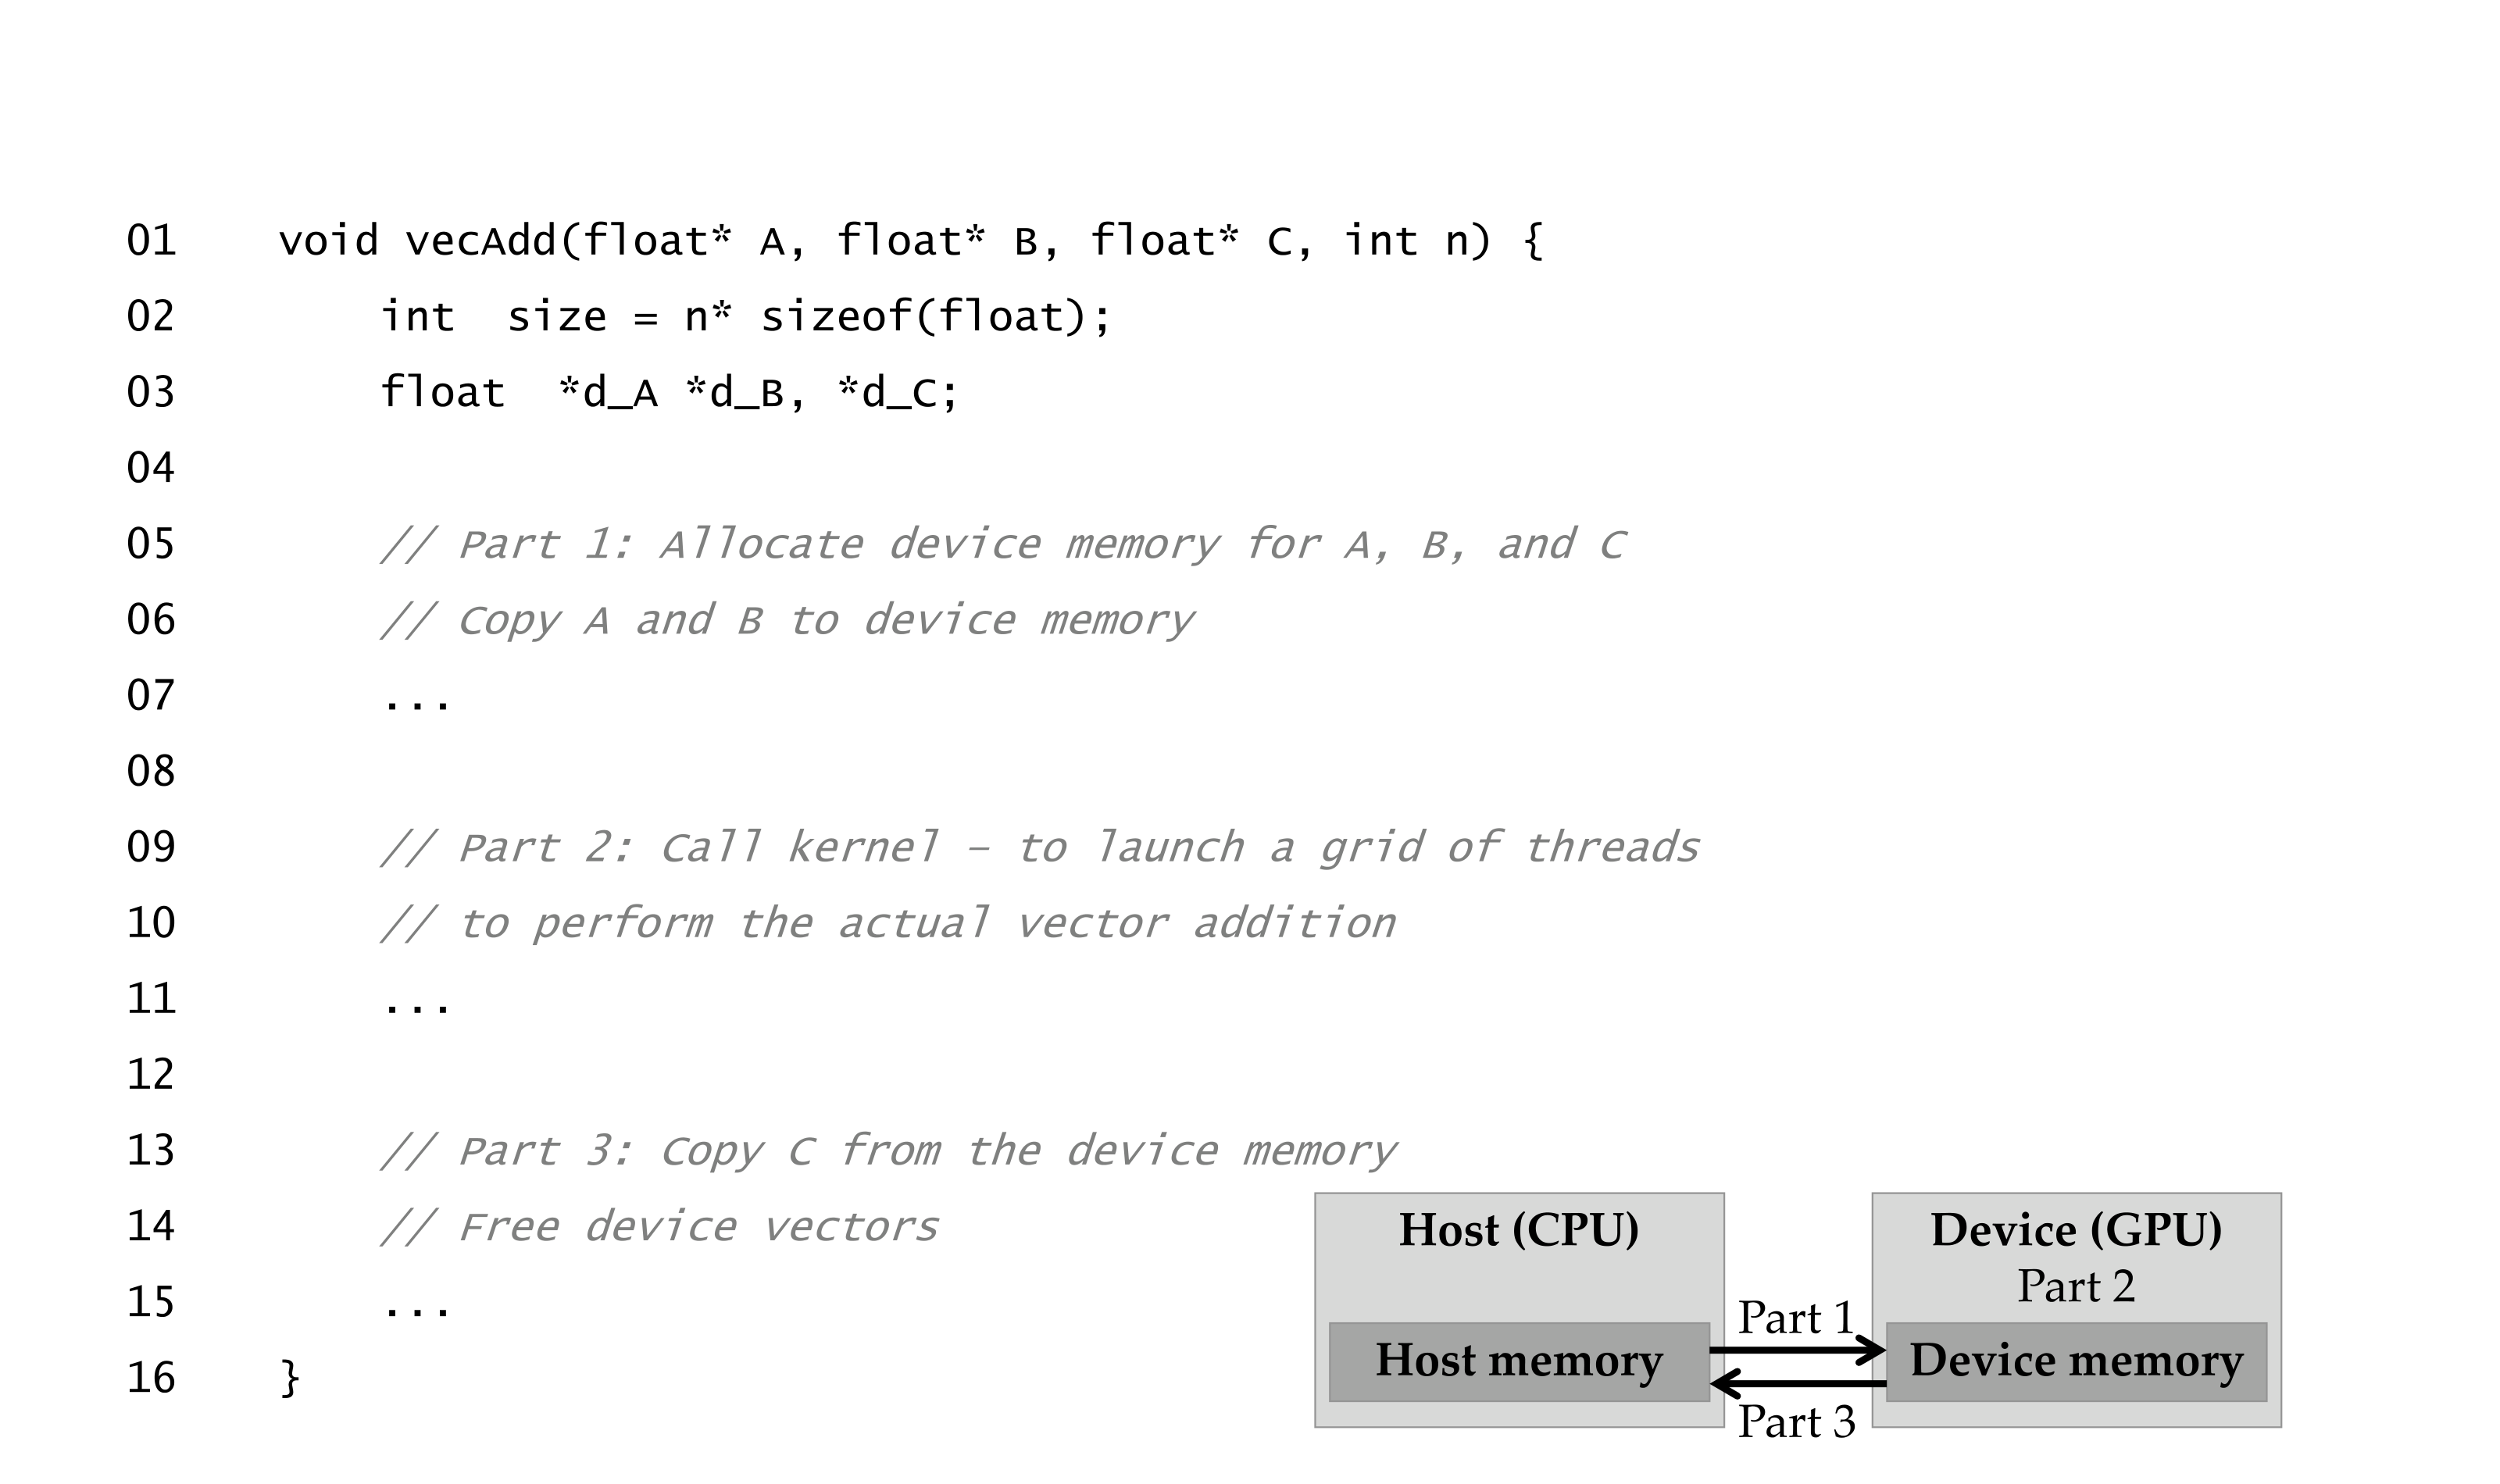
\includegraphics[width=\textwidth]{figs/ch2/2-5.png}
  \caption{把工作移到设备上的 \code{vecAdd}（主机代码）函数概要及数据流}
  \label{fig:2-5}
\end{figure}

修改后的 \code{vecAdd} 函数本质上是一个外包代理：它把输入数据发送到设备，在
设备上启动计算，再从设备收集结果，而且主程序甚至不需要知道向量加法实际上已经
在设备上完成。实践中，这种“透明”的外包模型可能非常低效，因为数据需要来回
复制。通常会把大型而重要的数据结构保留在设备上，只从主机代码调用操作这些数据
结构的设备函数。不过，目前为了介绍 CUDA C++ 程序的基本结构，我们先使用这个
简化的透明模型。修改后函数的细节，以及如何组成内核函数，将是本章后续内容。

\section{设备全局内存与数据传送}
\label{sec:device-global-memory}

在当前 CUDA 系统中，设备通常是配有自身动态随机存取存储器（Dynamic
Random-Access Memory，DRAM）的硬件卡；这块 DRAM 称为设备全局内存（device
global memory），通常简称全局内存。例如，NVIDIA Hopper H100 GPU 配备 80 GB
或 94 GB 全局内存。称其为“全局”内存，是为了区别于设备上其他同样可以由程序员
访问的内存类型。CUDA 内存模型和不同设备内存类型的细节将在第 5 章讨论。

对于向量加法内核，调用内核之前，程序员需要在设备全局内存中分配空间，并把数据
从主机内存传送到设备全局内存中的已分配空间。这些活动对应图 \ref{fig:2-5} 的
第 1 部分。设备执行结束后，程序员还需要把输出数据从设备全局内存传回主机内存，
并释放不再需要的设备全局内存空间；这些活动对应第 3 部分。\textcolor{red}{CUDA 运行时系统
（通常运行在主机上）提供 API 函数，代表程序员完成这些活动。}下文简称“从主机
向设备传送数据”，指把数据从主机内存复制到设备全局内存；反方向同理。

图 \ref{fig:2-5} 的第 1 和第 3 部分需要使用 CUDA API 函数，为 $A$、$B$、$C$
分配设备全局内存，把 $A$ 和 $B$ 从主机传到设备，在向量加法之后把 $C$ 从设备
传回主机，并释放 $A$、$B$、$C$ 所占的设备全局内存。先介绍内存分配和释放函数。

\begin{figure}[htbp]
  \centering
  \begin{tabular}{>{\ttfamily}p{0.22\textwidth} p{0.65\textwidth}}
    \toprule
    \code{cudaMalloc()} & 在设备全局内存中分配对象且需要两个参数。\\
    {\normalfont\bfseries 指针的地址：} & 该指针指向所分配对象。\\
    {\normalfont\bfseries 大小：} & 该分配对象以字节数表示的分配大小。\\
    \code{cudaFree()} & 从设备全局内存释放对象且需要一个参数。\\
    {\normalfont\bfseries 指针：} & 指向待释放对象。\\
    \bottomrule
  \end{tabular}
  \caption{管理设备全局内存的 CUDA API 函数（依据原书图 2.6 重绘）}
  \label{fig:2-6}
\end{figure}

图 \ref{fig:2-6} 展示了分配和释放设备全局内存的两个 API 函数。主机代码可以调用
\code{cudaMalloc}，\textbf{为对象分配一段设备全局内存}。读者应注意，\code{cudaMalloc}
与标准 C 运行时库（它也是 C++ 的一部分）中的 \code{malloc} 函数非常相似。这种
相似是有意的：CUDA C++ 只是带有少量扩展的 C++。CUDA C++ 使用标准 C/C++ 运行时
库的 \code{malloc} 函数管理主机内存，并添加 \code{cudaMalloc} 作为 C++ 运行时
库的扩展。尽量保持与原始 C/C++ 运行时库接近的接口，可以减少 C 或 C++ 程序员
重新学习这些扩展的时间。

\code{cudaMalloc} 的第一个参数，是将被设置为指向所分配对象的指针变量的地址。
这个地址本身是“指向指针的指针”；由于 API 的形参类型为 \code{void**}，调用者
需要把该地址转换为 \code{(void**)}。这个内存分配函数是通用函数，不局限于某种
对象类型。\footnote{\code{cudaMalloc} 通过通用指针交回所分配对象的地址，这会使
动态分配的多维数组使用起来更加复杂；第 3 章将讨论这一问题。} 无论指针变量是
什么类型，这个参数都允许 \code{cudaMalloc} 把所分配内存的地址写入提供的指针
变量。调用内核的主机代码会把这个指针值传给需要访问所分配内存对象的内核。第二个
参数给出要分配的数据大小，单位是字节；它与 C \code{malloc} 函数的大小参数一致。

注意，\code{cudaMalloc} 的格式与 C \code{malloc} 略有不同。C \code{malloc}
返回指向所分配对象的指针，只接收一个指定对象大小的参数；\code{cudaMalloc} 则
把结果写入第一个参数所指定地址的指针变量。因此，\code{cudaMalloc} 接收两个
参数。\textbf{双参数形式使 \code{cudaMalloc} 能像其他 CUDA API 函数一样，使用返回值
报告错误。}

\code{cudaFree} 函数与 C \code{free} 函数非常相似。它接收一个输入参数，即
待释放内存的指针，并\textbf{从设备内存中释放相应空间}。

CUDA C++ 还有更高级的库函数，用于在主机内存和设备内存中分配与释放空间。这些
替代方法可以更快地复制数据，或者消除显式复制的需要，让数据按需自动复制。管理
设备内存时，这些方法可以为程序提供更好的性能或便利性；第 23 章和附录 C 会讨论
其他内存分配形式。

下面用一个简单代码例子说明 \code{cudaMalloc} 和 \code{cudaFree} 的使用：

\begin{lstlisting}[language=C++]
float *A_d;
int size = n * sizeof(float);
cudaMalloc((void**)&A_d, size);
...
cudaFree(A_d);
\end{lstlisting}

这是图 \ref{fig:2-5} 示例的延续。为清晰起见，我们在指针变量名后加 \code{_d}，
表示它指向设备全局内存中的对象。\code{A_d} 的类型是 \code{float*}，所以它的
地址 \code{&A_d} 的类型是 \code{float**}；\code{cudaMalloc} 的第一个形参类型
是 \code{void**}，因此代码中的 \code{(void**)&A_d} 把 \code{float**} 转换为
\code{void**}。\code{cudaMalloc} 返回时，\code{A_d} 将指向为向量 $A$ 分配的
设备全局内存区域。第二个参数是要分配的区域大小。由于 \code{size} 的单位是字节，
程序员在确定 \code{size} 的值时，需要把数组元素数量换算成字节数。

例如，为包含 $n$ 个单精度浮点元素的数组分配空间时，\code{size} 等于 $n$ 乘以
单精度浮点数的大小；当前计算机中该大小通常是 4 字节。因此，\code{size} 的值
为 \code{n*4}。计算完成后，调用 \code{cudaFree} 并把 \code{A_d} 作为参数传入，
即可从设备全局内存中释放向量 $A$ 的存储空间。注意，\code{cudaFree} 不需要改变
\code{A_d} 的值；它只需使用 \code{A_d} 的值，把已分配内存归还到可用内存池。
因此，作为参数传入的只是 \code{A_d} 的值，而不是其地址。

\code{A_d}、\code{B_d} 和 \code{C_d} 中的地址都指向设备全局内存中的位置。这些
地址不应在主机代码中解引用，只能用于调用 API 函数和内核函数。\textbf{在主机代码中解引用
设备全局内存指针可能导致异常或其他运行时错误，因为这些地址位于设备全局内存，
用户主机代码无法访问。}

讨论完 \code{A_d} 指针变量的声明，以及它在 \code{cudaMalloc} 和 \code{cudaFree}
调用中的用法后，读者应当能够用类似声明为 \code{B_d}、\code{C_d} 的指针变量及
相应的 \code{cudaMalloc} 调用，补全图 \ref{fig:2-5} 中 \code{vecAdd} 示例的
第 1 部分；第 3 部分则可以用针对 \code{B_d} 和 \code{C_d} 的 \code{cudaFree}
调用补全。

主机代码为数据对象分配设备全局内存后，就可以请求在主机与设备之间传送数据。这
通过调用 CUDA API 函数完成。图 \ref{fig:2-7} 展示了这样的 API 函数
\code{cudaMemcpy}。它接收四个参数：第一个参数是待复制数据对象的目标地址；
第二个参数是源地址；第三个参数指定复制的字节数；第四个参数表示复制涉及的
内存位置：主机到主机、主机到设备、设备到主机或设备到设备。例如，内存复制函数
也可以把设备全局内存中的数据从一个位置复制到另一个位置。

\begin{figure}[htbp]
  \centering
  \begin{tabular}{>{\ttfamily}p{0.25\textwidth} p{0.62\textwidth}}
    \toprule
    \code{cudaMemcpy()} & 执行内存数据传送，需要四个参数。 \\
    {\normalfont \bfseries 目标指针} & 指向目标内存地址的指针。 \\
    {\normalfont \bfseries 源指针} & 指向源内存地址的指针。\\ 
    {\normalfont \bfseries 大小} & 要复制的字节数。\\
    {\normalfont \bfseries 传输类型} & 即传送方向。\\
    \bottomrule
  \end{tabular}
  \caption{在主机与设备之间传送数据的 CUDA API 函数}
  \label{fig:2-7}
\end{figure}

\code{vecAdd} 函数在相加之前调用 \code{cudaMemcpy}，把 \code{A_h} 和 \code{B_h}
所指向的主机数组复制到 \code{A_d} 和 \code{B_d} 所指向的设备数组；向量加法
完成后，再把 \code{C_d} 所指向的设备数组复制到 \code{C_h} 所指向的主机数组。
假设 \code{A_h}、\code{B_h}、\code{A_d}、\code{B_d} 和 \code{size} 的值都已按
前文设置好，三个 \code{cudaMemcpy} 调用如下：

\begin{lstlisting}[language=C++]
cudaMemcpy(A_d, A_h, size, cudaMemcpyHostToDevice);
cudaMemcpy(B_d, B_h, size, cudaMemcpyHostToDevice);
...
cudaMemcpy(C_h, C_d, size, cudaMemcpyDeviceToHost);
\end{lstlisting}

\code{cudaMemcpyHostToDevice} 和 \code{cudaMemcpyDeviceToHost} 是 CUDA 编程环境
能够识别的预定义符号常量。通过正确安排源指针和目标指针，并使用适当的传送类型，
同一个 \code{cudaMemcpy} 函数可以用于两个方向的数据传送。

总的来说，图 \ref{fig:2-4} 中的 \code{main} 函数调用同样在主机上执行的
\code{vecAdd}；图 \ref{fig:2-5} 概要展示的 \code{vecAdd} 在设备全局内存中
分配空间、请求数据传送，并调用真正执行向量加法的内核。\textbf{我们把这种用于调用内核
的主机代码称为内核调用存根（stub）}。图 \ref{fig:2-8} 给出了更完整版本的
\code{vecAdd} 函数。

\begin{figure}[htbp]
  \centering
  \begin{lstlisting}[language=C++]
void vecAdd(float* A_h, float* B_h, float* C_h, int n) {
    int size = n * sizeof(float);
    float *A_d, *B_d, *C_d;

    cudaMalloc((void**)&A_d, size);
    cudaMalloc((void**)&B_d, size);
    cudaMalloc((void**)&C_d, size);

    cudaMemcpy(A_d, A_h, size, cudaMemcpyHostToDevice);
    cudaMemcpy(B_d, B_h, size, cudaMemcpyHostToDevice);

    // The kernel invocation is introduced later
    ...

    cudaMemcpy(C_h, C_d, size, cudaMemcpyDeviceToHost);

    cudaFree(A_d);
    cudaFree(B_d);
    cudaFree(C_d);
}
  \end{lstlisting}
  \caption{更完整版本的 \code{vecAdd} 函数}
  \label{fig:2-8}
\end{figure}

与图 \ref{fig:2-5} 相比，图 \ref{fig:2-8} 中的 \code{vecAdd} 已经完成第 1 和
第 3 部分。第 1 部分为 \code{A_d}、\code{B_d}、\code{C_d} 分配设备全局内存，
并把 \code{A_h} 传到 \code{A_d}、把 \code{B_h} 传到 \code{B_d}；这是通过调用
\code{cudaMalloc} 和 \code{cudaMemcpy} 完成的。读者可以尝试使用适当的参数值
自行编写这些函数调用，并与图 \ref{fig:2-8} 中的代码比较。第 2 部分调用内核，
将在下一小节介绍。第 3 部分把向量和数据从设备传回主机，使 \code{main} 函数
能够使用这些值；这通过调用 \code{cudaMemcpy} 完成。随后通过调用 \code{cudaFree}
释放设备全局内存中 \code{A_d}、\code{B_d} 和 \code{C_d} 所占的空间。

\begin{quote}
\textbf{CUDA C++ 程序中的错误检查与处理}

程序检查并处理错误非常重要。良好的错误检查和处理能够在错误发生时捕获它们，
并在靠近问题根因的位置发现问题。CUDA API 函数会返回标志，指示其处理请求时
是否发生错误；大多数错误来自调用时使用了不恰当的参数值。为简洁起见，本书的
示例不展示错误检查代码。例如，图 \ref{fig:2-8} 中有如下 \code{cudaMalloc}
调用：
\[
\code{cudaMalloc((void **) &A_d, size);}
\]

实践中，CUDA 程序员会用检查返回错误条件的代码包围该调用，并打印相关错误消息，
让用户知道发生了错误。一个简单版本如下：

\begin{lstlisting}[language=C++]
cudaError_t err =
    cudaMalloc((void **) &A_d, size);
if (err != cudaSuccess) {
    printf("%s in %s at line %d \n",
           cudaGetErrorString(err), __FILE__,
           __LINE__);
    exit(EXIT_FAILURE);
}
\end{lstlisting}

这样，如果系统设备内存不足，用户就会得到通知。恰当的错误检查可以节省数小时的
调试时间；还可以定义 C++ 宏，使源代码中的检查代码更加简洁。\textcolor{red}{原书示例的条件
判断写作 \code{error}，但前一行声明的是 \code{err}；此处按上下文改为
\code{err}。}
\end{quote}

\section{内核函数与线程}
\label{sec:kernel-functions-and-threading}

现在可以进一步讨论 CUDA C++ 内核函数，以及调用这些内核函数所产生的效果。在
CUDA 中，内核函数规定了 GPU 线程在并行阶段执行的代码。由于所有线程执行相同
的代码，CUDA C++ 编程是著名的单程序多数据（Single-Program Multiple-Data，
SPMD）\cite{atallah1998} 并行编程风格的一个实例；SPMD 是并行计算系统中常见的
编程风格。

当程序的主机代码调用内核时，运行在主机上的 CUDA 运行时系统会启动一个 GPU
线程网格，线程网格按两级层次组织。每个网格都组织为线程块（thread block）数组；
为简洁起见，后文也简称为块（block）。同一网格中的所有块大小相同。在当前系统
中，每个块最多可以包含 1024 个线程。图 \ref{fig:2-9} 展示了每个块包含 256
个线程的例子；每个线程用一条弯曲箭头表示，箭头来自一个标有该线程在块内索引
编号的方框。

网格中的块数量以及每个块中的线程数量，由主机代码在调用内核时指定。同一个内核
可以在主机代码的不同位置以不同的块数和线程数调用。对于给定的线程网格，每个
块中的线程数保存在名为 \code{blockDim} 的内置变量中。\code{blockDim} 的类型
是一个 C++ 结构体，包含三个无符号整数字段 \code{x}、\code{y} 和 \code{z}，
帮助程序员把线程组织成一维、二维或三维数组。一维组织只使用 \code{x} 字段；
二维组织使用 \code{x} 和 \code{y} 字段；三维结构则使用全部三个字段。线程组织
的维度通常反映数据的维度。\textbf{由于线程是为并行处理数据而创建的，让线程组织方式
反映数据组织方式是自然的}。

\begin{figure}[htbp]
  \centering
  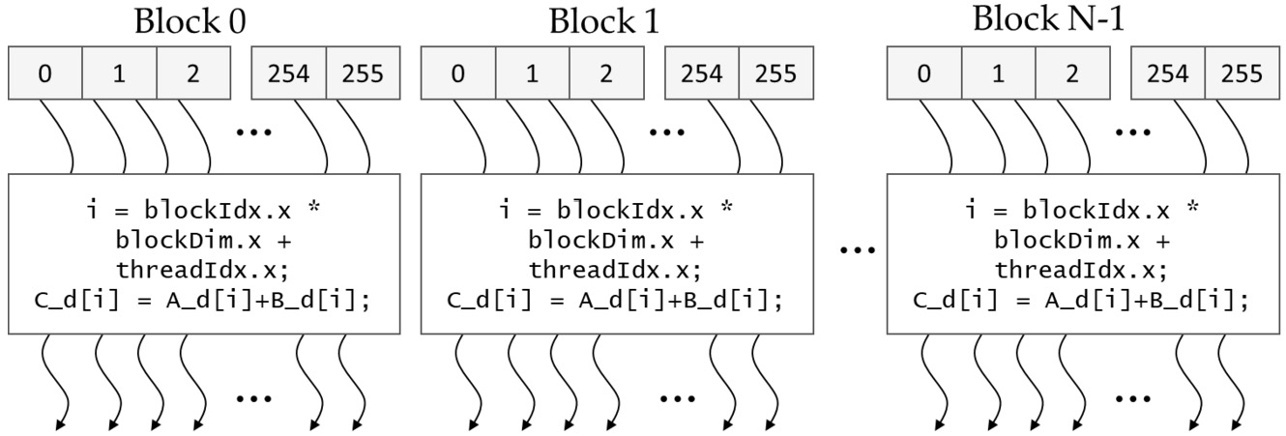
\includegraphics[width=\textwidth]{figs/ch2/2-9.png}
  \caption{网格中的所有线程执行相同的内核代码}
  \label{fig:2-9}
\end{figure}

\begin{quote}
\textbf{内置变量}

许多编程语言都有内置变量。这些变量具有特殊的含义和用途，通常由运行时系统
预先初始化，并且在程序中一般是只读的。程序员不应为了其他目的重新定义这些变量。
\end{quote}

在图 \ref{fig:2-9} 中，由于数据是一维向量，每个线程块都组织为一维线程数组。

每个块中的线程总数由内置变量 \code{blockDim.x} 给出。在图中，该值为 256。
\textbf{通常建议线程块中的线程总数是 32 的倍数}，这是出于硬件效率的考虑；本书后文会
再次讨论这一点。

CUDA 内核还可以访问另外两个内置变量 \code{threadIdx} 和 \code{blockIdx}，让
线程彼此区分，并确定每个线程需要处理的数据区域。\code{threadIdx} 为每个线程
提供块内的唯一坐标。在一维线程组织中只使用 \code{threadIdx.x}；图
\ref{fig:2-9} 中每个线程的小阴影方框显示了它的 \code{threadIdx.x} 值。每个块
中的第一个线程的值为 0，第二个线程的值为 1，第三个线程的值为 2，以此类推。

\code{blockIdx} 为一个块中的所有线程提供共同的块坐标。在图 \ref{fig:2-9} 中，
第一个块的所有线程的 \code{blockIdx.x} 值为 0，第二个块的值为 1，以此类推。
可以用电话系统作类比：\code{threadIdx.x} 类似本地电话号码，\code{blockIdx.x}
类似区号。两者结合起来，就能为全国范围内的每条电话线形成唯一的电话号码。同样，
每个线程也可以组合自己的 \code{threadIdx} 和 \code{blockIdx} 值，在整个网格
中生成唯一的全局索引。

\begin{quote}
\textbf{层次化组织}

像 CUDA 线程一样，现实世界中的许多系统也按层次组织。美国电话系统就是一个好
例子。最高层由许多“区域”组成，每个区域对应一个地理范围；同一区域内的所有
电话线共享一个三位数区号。一个电话区域有时会大于一座城市。例如，美国伊利诺伊
州中部的许多县和城市都属于同一电话区域，共享区号 217。

在一个区域内，每条电话线都有一个七位数的本地号码，因此每个区域最多约有一千万
个号码。可以把每条电话线看作一个 CUDA 线程，把区号看作 \code{blockIdx}，把
七位本地号码看作 \code{threadIdx}。这种层次化组织在保持局部性的同时，支持非常
大的电话线路数量；\textcolor{red}{拨打同一区域的号码时只需拨本地号码，偶尔拨打其他区域的号码
时才需要拨 1、区号和本地号码}。CUDA 线程的层次化组织也提供了一种局部性形式，
本书很快就会研究这种局部性。
\end{quote}

在图 \ref{fig:2-9} 中，使用下面的 C++ 语句计算唯一的全局索引 $i$：
\[
  i = \code{blockIdx.x} \times \code{blockDim.x} + \code{threadIdx.x}.
\]
本例中 \code{blockDim.x} 为 256。块 0 中线程的 $i$ 值范围为 0 到 255；块 1
中的范围为 256 到 511；块 2 中的范围为 512 到 767。也就是说，这三个块中线程
的 $i$ 值连续覆盖 0 到 767。由于每个线程使用 $i$ 访问 $A$、$B$ 和 $C$，这些
线程覆盖原始循环的前 768 次迭代。启动包含更多块的网格，就可以处理更长的向量；
启动包含 $n$ 个或更多线程的网格，就可以处理长度为 $n$ 的向量。

图 \ref{fig:2-10} 展示了向量加法的内核函数。注意，内核代码不采用 \code{_h} 和
\code{_d} 后缀约定，因为这里不存在混淆的可能；本章示例的内核代码不会访问任何
主机内存。\footnote{一般来说，内核代码可以通过称为统一虚拟地址（Unified
Virtual Address，UVA）的机制访问主机内存。该机制允许 GPU 访问主机内存，但带宽
低于访问自身设备全局内存；附录 C 会讨论这一机制。}

\begin{figure}[htbp]
  \centering
  \begin{lstlisting}[language=C++]
// Compute vector sum C = A + B
// Each thread performs one pair-wise addition
__global__
void vecAddKernel(float* A, float* B, float* C, int n) {
    int i = threadIdx.x + blockDim.x * blockIdx.x;
    if (i < n) {
        C[i] = A[i] + B[i];
    }
}
  \end{lstlisting}
  \caption{一个简单的向量加法内核函数}
  \label{fig:2-10}
\end{figure}

内核的语法遵循 C++ 标准，但有一些值得注意的扩展。首先，在
\code{vecAddKernel} 声明前有 CUDA 专用关键字 \code{__global__}。该关键字表示
这是一个内核，可以被调用来在设备上生成线程网格。

一般而言，CUDA C++ 用三个限定符关键字扩展 C++ 语言，可以在函数声明中使用。
图 \ref{fig:2-11} 总结了这些关键字的含义。\code{__global__} 表示所声明的
函数是 CUDA C++ 内核函数。注意，单词 \code{global} 两侧各有两个下划线。这种
内核函数在设备上执行，可以从主机调用；在支持动态并行性的 CUDA 系统中（从
Kepler 架构开始），也可以从设备调用。重要特征是，调用这种内核函数会在设备，
即 GPU 上启动一个新的线程网格。

\begin{figure}[htbp]
  \centering
  \begin{tabular}{>{\ttfamily}p{0.20\textwidth} p{0.18\textwidth} p{0.18\textwidth} p{0.28\textwidth}}
    \toprule
    限定符关键字 & 可从哪里调用 & 在哪里执行 & 由谁执行 \\
    \midrule
    \code{__host__}（默认） & 主机 & 主机 & 调用者主机线程 \\
    \code{__global__} & 主机（或设备） & 设备 & 新的设备线程网格 \\
    \code{__device__} & 设备 & 设备 & 调用者设备线程 \\
    \bottomrule
  \end{tabular}
  \caption{CUDA C++ 函数声明关键字}
  \label{fig:2-11}
\end{figure}

\code{__device__} 关键字表示所声明的是 CUDA 设备函数。设备函数在 GPU 设备上
执行，只能从内核函数或另一个设备函数中调用；它由调用它的设备线程执行，不会
启动新的设备线程。

\code{__host__} 关键字表示所声明的是 CUDA 主机函数。主机函数就是在主机上执行
的传统 C++ 函数，只能从另一个主机函数调用。如果声明中没有 CUDA 关键字，CUDA
程序中的所有函数默认都是主机函数。这很合理，因为许多 CUDA 应用是从只运行在
CPU 上的环境移植而来的；移植时，程序员会加入内核函数和设备函数，而原有函数
保持为主机函数。让函数默认成为主机函数，可以免去程序员修改所有原有函数声明
的繁琐工作。

既然所有函数默认都是主机函数，为什么还需要 \code{__host__} 关键字？有时，程序
员希望一个函数同时能够在主机和设备上使用。标记 \code{__device__} 会使函数只
在设备上可用；要让它在两者上都可用，可以在函数声明中同时使用 \code{__host__}
和 \code{__device__}。这种组合会告诉编译系统，为同一个函数生成两份目标代码：
一份在主机上执行，只能从主机函数调用；另一份在设备上执行，只能从设备函数或
内核函数调用。当同一份函数源代码需要重新编译以生成设备版本时，这种能力非常
有用，许多用户库函数可能属于这一类。

图 \ref{fig:2-10} 中 \code{vecAdd} 内核使用的第二个值得注意的 CUDA C++ 扩展，
是内置变量 \code{threadIdx}、\code{blockIdx} 和 \code{blockDim}。回顾一下，
所有线程执行相同的内核代码，因此必须有办法让线程彼此区分，并把每个线程导向
数据的特定部分。这些内置变量让线程能够访问硬件寄存器，从而获得标识自身的坐标。
不同线程会看到其 \code{threadIdx.x}、\code{blockIdx.x} 和 \code{blockDim.x}
变量的不同值。

利用内置变量计算出的全局索引（图 \ref{fig:2-10} 第 5 行）被写入一个类型为
\code{int} 的自动（局部）变量 $i$。\footnote{不同的 C 和 C++ 程序员在声明用于
表示数组索引、数组大小、循环迭代计数器和循环边界的变量时，可能选择 \code{int}
或 \code{unsigned int}。使用 \code{unsigned int} 能明确表明这些变量绝不应为
负数，并可能触发有助于防止错误的编译器警告。另一方面，在执行减法，或在算术
运算中混用 \code{unsigned int} 与其他 \code{int} 变量时，使用 \code{int} 可以
避免错误。此外，由于 \code{int} 溢出的行为未定义，编译器可以在优化时利用这一
事实。本书在上述声明中有时使用 \code{int}，有时使用 \code{unsigned int}；读者
在自己的实现中可采用任一种风格。} \textbf{在 CUDA 内核函数中，自动变量对每个线程都是
私有的。}
也就是说，每个线程都会生成一份 $i$；如果网格启动了 10,000 个线程，就会有
10,000 份 $i$，每个线程一份。一个线程赋给自己 $i$ 的值，其他线程不可见。本书
第 5 章会更详细地讨论这些自动变量。

比较图 \ref{fig:2-4} 和图 \ref{fig:2-10}，可以发现 CUDA 内核有一个重要特点：
图 \ref{fig:2-10} 中没有对应原始循环的 \code{for} 循环。读者可能会问，循环
去哪儿了？答案是，循环现在被线程网格替代。整个网格构成循环的等价物，网格中的
每个线程对应原始循环的一次迭代。这有时称为循环并行性，即把原来顺序代码的迭代
交给线程并行执行。

注意，\code{vecAddKernel} 中有 \code{if (i < n)}。这是因为并非所有向量长度都
能表示为块大小的整数倍。例如，向量长度为 100，最小的高效线程块维度为 32，
选择块大小 32 时，需要启动 4 个线程块才能处理全部 100 个向量元素。然而，4 个
块共包含 128 个线程；必须禁止最后 28 个线程执行原程序没有要求的工作。由于所有
线程执行相同代码，它们都会把自己的 $i$ 值与 $n=100$ 比较。借助
\code{if (i < n)}，前 100 个线程执行加法，最后 28 个线程不执行，从而允许内核
处理任意长度的向量。

\section{调用内核函数}
\label{sec:calling-kernel-functions}

实现内核函数后，下一步是在主机代码中调用它，以启动线程网格。图
\ref{fig:2-12} 展示了调用向量加法内核的主机代码。当主机代码调用内核时，会
通过执行配置参数设置网格和线程块的维度。配置参数放在传统 C++ 函数参数之前的
\code{<<<} 和 \code{>>>} 括号之间。第一个配置参数给出网格中的块数，第二个
参数指定每个块中的线程数；本例中每个块有 256 个线程。

\begin{figure}[htbp]
  \centering
  \begin{lstlisting}[language=C++]
void vecAdd(float* A, float* B, float* C, int n) {
    // Allocation and copying of A_d, B_d, and C_d omitted
    ...
    // Launch ceil(n/256) blocks with 256 threads per block
    vecAddKernel<<<ceil(n/256.0), 256>>>(A_d, B_d, C_d, n);
}
  \end{lstlisting}
  \caption{包含向量加法内核调用语句的主机代码示例}
  \label{fig:2-12}
\end{figure}


为了保证网格中的线程足以覆盖所有向量元素，需要把网格块数设置为所需线程数
（这里是 $n$）除以线程块大小（这里是 256）后的向上取整，即天花板除法。实现
天花板除法有很多方法；一种方法是对 \code{n/256.0} 应用 C++ 的 \code{ceil}
函数。使用浮点数 256.0 可以确保除法结果为浮点值，使 \code{ceil} 能正确向上
取整。例如，要生成 1000 个线程，就启动
\[
  \code{ceil(1000/256.0)}=4
\]
个线程块，结果是 $4\times256=1024$ 个线程。结合内核中的
\code{if (i < n)}，前 1000 个线程会对 1000 个向量元素执行加法，其余 24 个
线程不执行。

图 \ref{fig:2-13} 展示了 \code{vecAdd} 函数中的最终主机代码；它补全了图
\ref{fig:2-5} 中的骨架代码。图 \ref{fig:2-10} 和图 \ref{fig:2-13} 共同展示
了一个同时包含主机代码和设备内核的简单 CUDA 程序。

\begin{figure}[htbp]
  \centering
  \begin{lstlisting}[language=C++]
void vecAdd(float* A, float* B, float* C, int n) {
    float *A_d, *B_d, *C_d;
    int size = n * sizeof(float);

    cudaMalloc((void**)&A_d, size);
    cudaMalloc((void**)&B_d, size);
    cudaMalloc((void**)&C_d, size);

    cudaMemcpy(A_d, A, size, cudaMemcpyHostToDevice);
    cudaMemcpy(B_d, B, size, cudaMemcpyHostToDevice);

    vecAddKernel<<<ceil(n/256.0), 256>>>(A_d, B_d, C_d, n);

    cudaMemcpy(C, C_d, size, cudaMemcpyDeviceToHost);

    cudaFree(A_d);
    cudaFree(B_d);
    cudaFree(C_d);
}
  \end{lstlisting}
  \caption{向量加法内核调用语句}
  \label{fig:2-13}
\end{figure}

这份源代码把线程块大小硬编码为每块 256 个线程，但使用的线程块数量取决于向量
长度 $n$。如果 $n=750$，就使用 3 个线程块；如果 $n=4000$，就使用 16 个线程
块；如果 $n=2{,}000{,}000$，就使用 7813 个线程块。注意，所有线程块都操作
向量的不同部分，可以按任意顺序执行。\textbf{程序员不能对执行顺序作任何假设}。

执行资源较少的小型 GPU 可能一次只并行执行其中一两个线程块；较大的 GPU 可能
同时执行 128 或 256 个线程块。这使 CUDA 内核的执行速度能够随硬件扩展：同一份
代码在小型 GPU 上以较低速度运行，在大型 GPU 上以较高速度运行。第 4 章会再次
讨论这一点。

\section{编译}
\label{sec:compilation}

我们已经看到，实现 CUDA C++ 内核需要使用并非 C++ 标准组成部分的各种扩展。一旦
代码中使用了这些扩展，就不能再交给传统 C++ 编译器；必须使用能够识别和理解这些
扩展的编译器，例如 NVCC（NVIDIA CUDA Compiler）。

如图 \ref{fig:2-14} 顶部所示，NVCC 处理 CUDA C++ 程序，并利用 CUDA 关键字把
主机代码和设备代码分离。主机代码是普通 C++ 代码，由标准 C/C++ 编译器编译，
并作为传统 CPU 进程运行。标记了 CUDA 关键字、用于声明 CUDA 内核及其相关设备
函数和数据结构的设备代码，则由 NVCC 编译为称为 PTX 的虚拟二进制文件。随后，
NVCC 的运行时组件会进一步把这些 PTX 文件编译为真正的目标文件，并在支持 CUDA
的 GPU 设备上执行。

\begin{figure}[htbp]
  \centering
  \begin{tabular}{c}
    \textbf{包含 CUDA 扩展的 C++ 程序}\\
    $\downarrow$\\
    \fbox{\parbox{0.55\textwidth}{\centering NVCC 编译器}}\\[0.4em]
    \begin{tabular}{c@{\qquad}c}
      $\swarrow$ 主机代码 & 设备代码（PTX） $\searrow$\\
      \fbox{\parbox{0.31\textwidth}{\centering 主机 C++ 预处理器、编译器/链接器}}
      &
      \fbox{\parbox{0.31\textwidth}{\centering 设备即时编译器}}\\
      $\searrow$ & $\swarrow$
    \end{tabular}\\[0.4em]
    \fbox{\parbox{0.65\textwidth}{\centering 包含 CPU 和 GPU 的异构计算平台}}
  \end{tabular}
  \caption{CUDA C++ 程序的编译过程概览}
  \label{fig:2-14}
\end{figure}

\section{小结}
\label{sec:chapter-2-summary}

本章快速、简化地概览了 CUDA C++ 编程模型。CUDA C++ 扩展 C++ 语言以支持并行
计算，本章讨论了这些扩展中的一个基本子集。为方便读者，现将这些扩展总结如下。

\paragraph{函数声明。}
CUDA C++ 扩展 C++ 函数声明语法，以支持异构并行计算。图 \ref{fig:2-11} 总结了
这些扩展。使用 \code{__global__}、\code{__device__} 或 \code{__host__} 中的
一个，程序员可以指示编译器生成内核函数、设备函数或主机函数。没有这些关键字的
函数声明默认是主机函数。如果函数声明同时使用 \code{__host__} 和
\code{__device__}，编译器会生成两个版本，一个用于设备，一个用于主机。

\paragraph{内核调用与网格启动。}
CUDA C++ 用被 \code{<<<} 和 \code{>>>} 括号包围的内核执行配置参数扩展 C++
函数调用语法。这些执行配置参数只在调用内核函数、启动线程网格时使用。本章讨论
了定义网格维度和每个块维度的执行配置参数；关于内核启动扩展以及其他类型执行
配置参数的更多细节，请参阅 CUDA 编程指南 \cite{cuda2025-ch2}。

\paragraph{内置（预定义）变量。}
CUDA 内核可以访问一组内置只读变量，让每个线程区分自己与其他线程，并确定自己
需要处理的数据区域。本章讨论了 \code{threadIdx}、\code{blockDim} 和
\code{blockIdx}；第 3 章将进一步讨论如何使用这些变量，在处理多维数据时管理
多维块和网格。

\paragraph{运行时 API。}
CUDA 支持一组应用程序接口（Application Programming Interface，API）函数，为
CUDA C++ 程序提供服务。本章讨论的服务包括 \code{cudaMalloc}、\code{cudaFree}
和 \code{cudaMemcpy}；这些函数由主机代码调用，分别代表调用程序分配设备全局
内存、释放设备全局内存，以及在主机和设备之间传送数据。关于其他 CUDA API 函数，
请参阅 CUDA C++ 编程指南 \cite{cuda2025-ch2}。

本章的目标是介绍 CUDA C++ 的核心概念，以及编写简单 CUDA 程序所需的基本 CUDA
到 C++ 的扩展。本章绝不是 CUDA 全部特性的完整说明；本书后续部分还会介绍更多
特性。不过，我们强调的是这些特性所支持的关键并行计算概念。对于并行编程技术
的代码示例，我们只会介绍足够使用的 CUDA C++ 特性。一般而言，我们始终建议
读者查阅 CUDA C++ 编程指南 \cite{cuda2025-ch2}，了解最新特性的更多细节。

\section{练习}
\label{sec:chapter-2-exercises}

\begin{enumerate}[label=\arabic*.,leftmargin=2.7em]
  \item 如果希望网格中的每个线程计算向量加法的一个输出元素，那么在内核函数中，
  把线程/块索引映射到数据索引 $i$ 的表达式是什么？
  \begin{enumerate}[label=\alph*.,leftmargin=2.2em]
    \item \code{i = threadIdx.x + threadIdx.y;}
    \item \code{i = blockIdx.x + threadIdx.x;}
    \item \code{i = blockIdx.x * blockDim.x + threadIdx.x;}
    \item \code{i = blockIdx.x * threadIdx.x;}
  \end{enumerate}

  \item 假设希望每个线程计算向量加法中相邻的两个元素。把线程/块索引映射到线程
  要处理的第一个元素的数据索引 $i$ 的表达式是什么？
  \begin{enumerate}[label=\alph*.,leftmargin=2.2em]
    \item \code{i = blockIdx.x * blockDim.x + threadIdx.x + 2;}
    \item \code{i = blockIdx.x * threadIdx.x * 2;}
    \item \code{i = (blockIdx.x * blockDim.x + threadIdx.x) * 2;}
    \item \code{i = blockIdx.x * blockDim.x * 2 + threadIdx.x;}
  \end{enumerate}

  \item 希望每个线程计算两个元素。每个线程块处理由两个区段组成的、连续的
  $2\times\code{blockDim.x}$ 个元素。块中的所有线程先处理第一个区段，每个线程
  处理一个元素；然后它们一起移动到下一个区段，每个线程再处理一个元素。假设
  变量 $i$ 是线程要处理的第一个元素的索引，那么把线程/块索引映射到第一个
  元素数据索引的表达式是什么？
  \begin{enumerate}[label=\alph*.,leftmargin=2.2em]
    \item \code{i = blockIdx.x * blockDim.x + threadIdx.x + 2;}
    \item \code{i = blockIdx.x * threadIdx.x * 2;}
    \item \code{i = (blockIdx.x * blockDim.x + threadIdx.x) * 2;}
    \item \code{i = blockIdx.x * blockDim.x * 2 + threadIdx.x;}
  \end{enumerate}

  \item 对于一次向量加法，向量长度为 8000，每个线程计算一个输出元素，线程块
  大小为 1024。程序员把内核调用配置为覆盖所有输出元素所需的最少线程块数。
  网格中有多少个线程？
  \begin{enumerate}[label=\alph*.,leftmargin=2.2em]
    \item 8000
    \item 8196
    \item 8192
    \item 8200
  \end{enumerate}

  \item 要为包含 $v$ 个整数元素的数组分配设备全局内存。
  \code{cudaMalloc} 的第二个参数应使用哪个表达式？
  \begin{enumerate}[label=\alph*.,leftmargin=2.2em]
    \item \code{n}
    \item \code{v}
    \item \code{n * sizeof(int)}
    \item \code{v * sizeof(int)}
  \end{enumerate}

  \item 如果希望分配一个包含 $n$ 个浮点元素的数组，并让浮点指针变量
  \code{A_d} 指向所分配的内存，\code{cudaMalloc} 调用的第一个参数应使用什么
  表达式？
  \begin{enumerate}[label=\alph*.,leftmargin=2.2em]
    \item \code{n}
    \item \code{(void *) A_d}
    \item \code{*A_d}
    \item \code{(void **) &A_d}
  \end{enumerate}

  \item 如果希望把 3000 字节数据从主机数组 \code{A_h}（\code{A_h} 指向源数组
  的第 0 个元素）复制到设备数组 \code{A_d}（\code{A_d} 指向目标数组的第 0 个
  元素），CUDA 中适合进行该复制的 API 调用是什么？
  \begin{enumerate}[label=\alph*.,leftmargin=2.2em]
    \item \code{cudaMemcpy(3000, A_h, A_d, cudaMemcpyHostToDevice);}
    \item \code{cudaMemcpy(A_h, A_d, 3000, cudaMemcpyDeviceToHost);}
    \item \code{cudaMemcpy(A_d, A_h, 3000, cudaMemcpyHostToDevice);}
    \item \code{cudaMemcpy(3000, A_d, A_h, cudaMemcpyHostToDevice);}
  \end{enumerate}

  \item 应如何声明变量 \code{err}，才能适当地接收 CUDA API 调用返回的值？
  \begin{enumerate}[label=\alph*.,leftmargin=2.2em]
    \item \code{int err;}
    \item \code{cudaError err;}
    \item \code{cudaError_t err;}
    \item \code{cudaSuccess_t err;}
  \end{enumerate}

  \item 考虑图 \ref{fig:2-15} 中的 CUDA 内核及调用它的主机函数。

  \begin{figure}[htbp]
    \centering
    \begin{lstlisting}[language=C++]
__global__ void foo_kernel(float* a, float* b, unsigned int N) {
    unsigned int i = blockIdx.x * blockDim.x + threadIdx.x;
    if (i < N) {
        b[i] = 2.7f * a[i] - 4.3f;
    }
}
void foo(float* a_d, float* b_d) {
    unsigned int N = 200000;
    foo_kernel<<<(N + 128 - 1)/128, 128>>>(a_d, b_d, N);
}
    \end{lstlisting}
    \caption{练习题 9 的 CUDA 代码}
    \label{fig:2-15}
  \end{figure}

  \begin{enumerate}[label=\alph*.,leftmargin=2.2em]
    \item 每个块中的线程数是多少？
    \item 网格中的线程总数是多少？
    \item 网格中的块数是多少？
    \item 执行第 02 行代码的线程数是多少？
    \item 执行第 04 行代码的线程数是多少？
  \end{enumerate}

  \item 一位新的 CUDA 程序员对 CUDA 感到沮丧。他抱怨 CUDA 太繁琐：自己计划
  在主机和设备上都执行的许多函数，必须分别声明两次，一次声明为主机函数，一次
  声明为设备函数。你会如何帮助这位新程序员？
\end{enumerate}

\begin{chapterbibliography}{3}

\bibitem{patt2020}
Y. N. Patt and S. J. Patel.
\emph{Introduction to Computing Systems: From Bits and Gates to C and Beyond}.
McGraw Hill Publisher, 2020, 2000, 2004.

\bibitem{atallah1998}
M. J. E. Atallah.
\emph{Algorithms and Theory of Computation Handbook}.
CRC Press, 1998.

\bibitem{cuda2025-ch2}
NVIDIA.
\emph{CUDA C++ Programming Guide}, Release 13.0, 2025.
\url{https://docs.nvidia.com/cuda/cuda-c-programming-guide}.

\end{chapterbibliography}
